%!TEX root = ../report.tex

\documentclass[../report.tex]{subfiles}
\begin{document}

\subsection{Potential Uses of Percolation in The Firefighter Problem}

We have identified three main avenues that may be pursued in {\scshape Firefighter} using Percolation: the firefighter may use percolation in order to defend the graph, the fire might spread with percolation probability $p$ or we might use percolation on the graph to form a more useful model (i.e. one that can more accurately represent an irregular population density). The former might be used when the firefighter can save more than one vertex at each turn; the latter may be more useful when modelling disease spread.
\begin{figure}[ht]
	\centering
		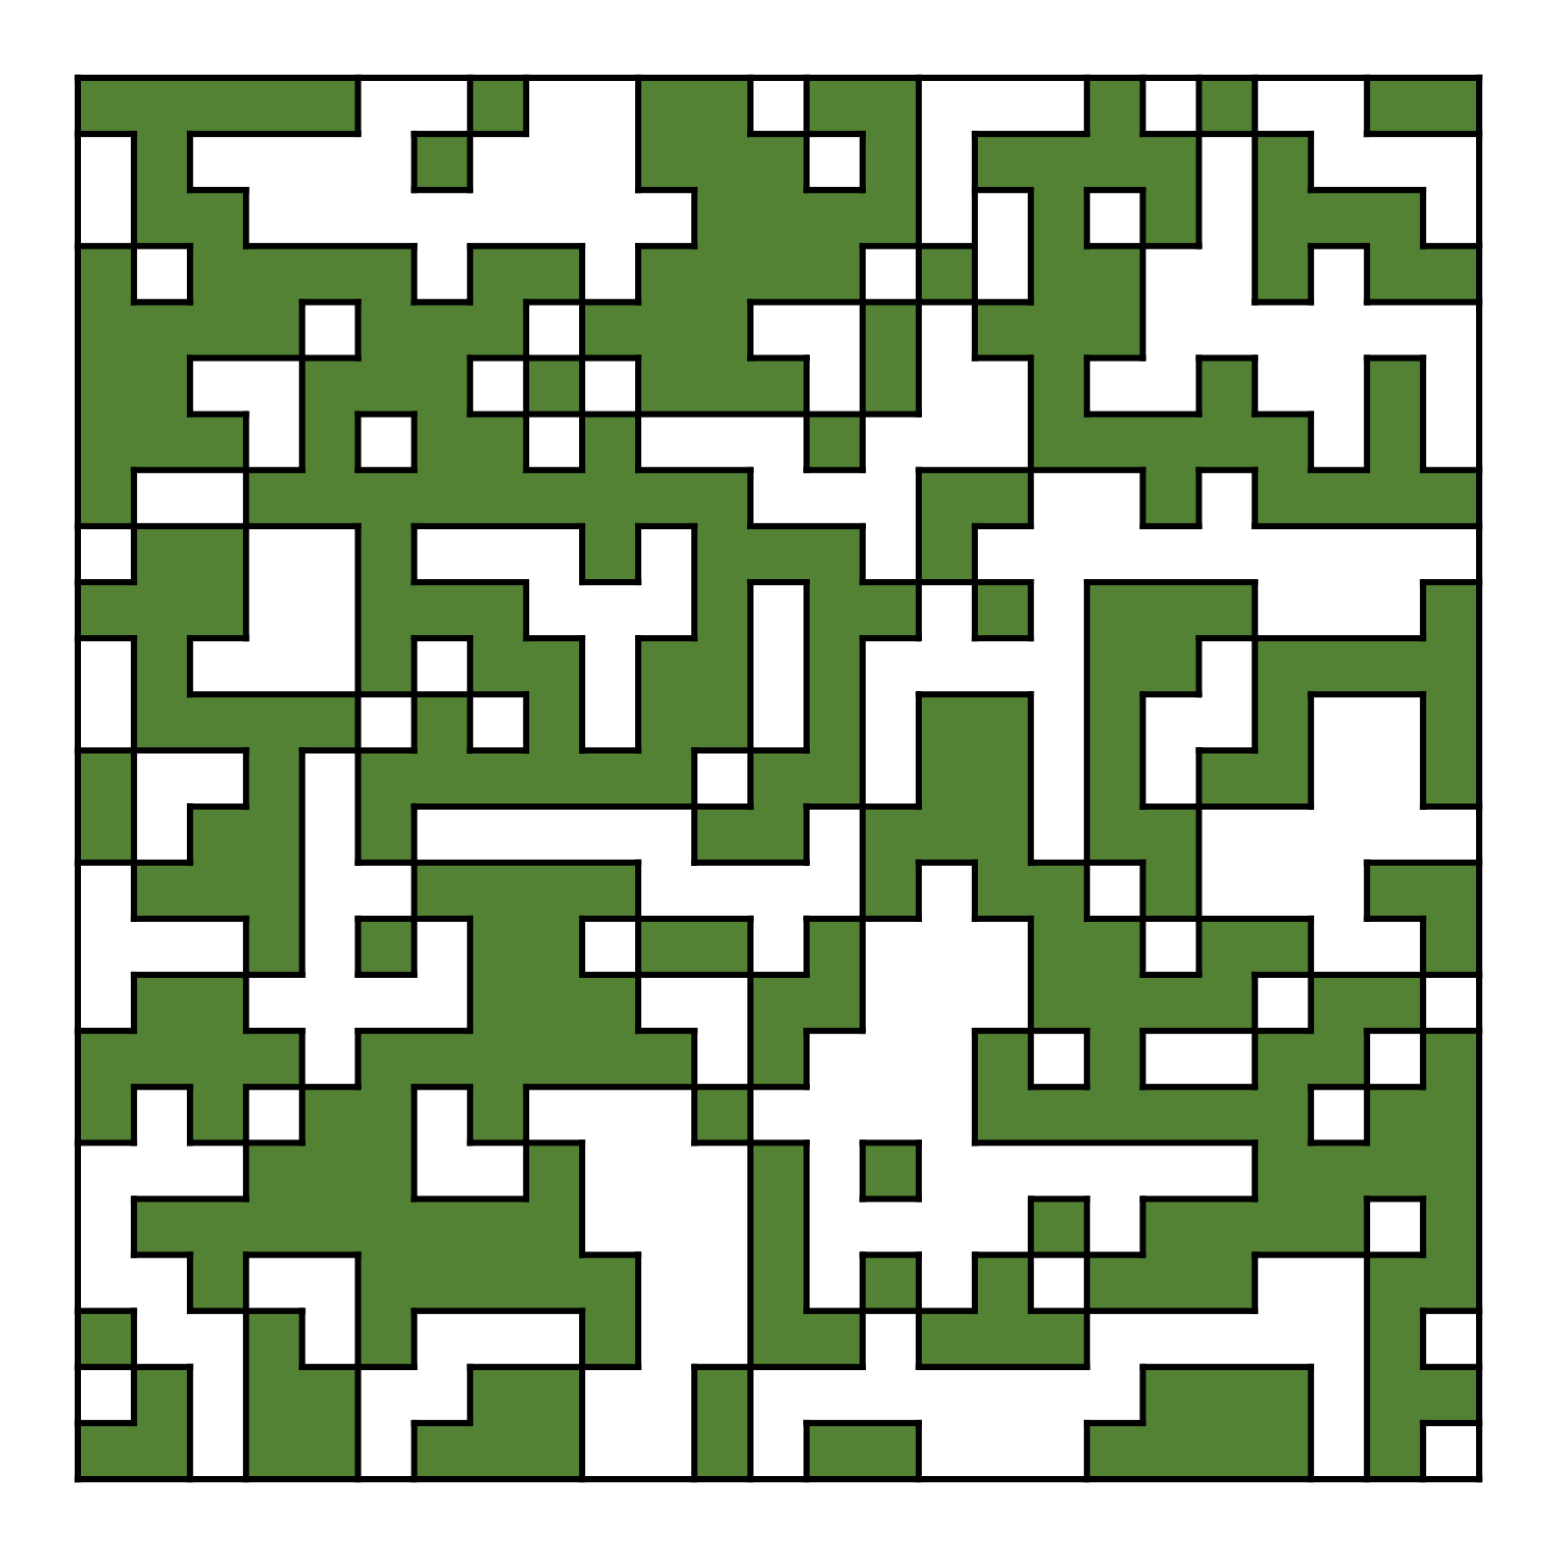
\includegraphics[width=0.3\linewidth]{firebreak/25x25/25x25}
	\caption{A regular $(25\times25)$ graph, percolated with probability $p=2/3$.}
	\label{fig:largeperc}
\end{figure}

%%%%%%%%%%

\subsubsection{Better than random}
One potential use for the firefighter using percolation as a method of defence would be as a baseline test: in most scenarios, a method for obtaining defence strategies should be at least as effective as a random defence sequence. We could find such a random sequence using percolation for comparison purposes. Consider a sequence of vertices in graph $G$, written as $d_1, d_2,\dots, d_t$. An optimal defence sequence could be found using integer programming as provided by Finbow and MacGillivray \cite{finbow_2009}:
\begin{equation*}
	\begin{array}{ll@{}ll}
\text{Maximise}  & \displaystyle \sum\limits_{v\in V(G)} d_v w(v) &\text{~for each level~} i\\
\text{subject to}& d_v + \displaystyle\sum\limits_{\text{level}(v)=i} d_v \leq 1  &\text{~for each level~} i\\
				 & d_v + \displaystyle\sum\limits_{u\succ v}  d_u \leq 1  &\text{~for every outer vertex~} v \text{~of~} T,\\
                 &d_{v} \in \{0,1\}. &
	\end{array}
\end{equation*}
where $u\succ v$ indicates that $u$ is an ancestor of $v$. The optimal strategies provided for different classes and densities of graphs here will provide an upper bound (which may indeed be impossible to attain in some cases) for success of a given strategy. We can find a lower bound using percolation, and so we have a range of success values as a starting point: if some strategy is better than random percolation, then it is worth considering, but below the particular expected optimal solution from integer programming and we can improve or find a better strategy.\\

We conjecture that, at the lowest graph densities, the random strategy will be very close to the optimal strategy and thus finding an improvement is at once difficult and lacking in great utility. At the very highest graph densities, while random strategies will have a very low expected best-case scenario, as will most strategies as the constraint on the firefighter that they have only one vertex to save per turn does not go as far when vertices are much better connected. Thus, finding improvements on random will again not prove very useful as random and best-case scenarios serve to show us that there is a small range of possible, not good outcomes.

\subsubsection{Reproduction rate}
We now focus our attention on the fire spread being determined by percolation (rather than the firefighter's defence sequence). Diseases, when there is a large enough sample size, have a basic reproduction rate associated with them, denoted $R_0$: for instance, measles has a basic reproduction rate $12\leq R_0 \leq 18$ \cite{guerra_2017} and the Influenza strain responsible for the 1918 pandemic has a basic reproduction rate of $1.4 \leq R_0 \leq 2.8$ \cite{ferguson_2006}. These baseline, theoretical values can be implemented as an internal probability to a propagating fire: to formulate a stochastic version of {\scshape Firedfighter}, we let the fire propagate with some probability (which could be determined by reproduction rate of a real infectious disease) in a percolation-like process and examine the change to optimal defence.

Where we wish to consider vertices as individuals and edges as the connections between them, percolation may give us a more useful model for disease spread when we do not assume the population is well mixed and instead introduce probability functions to correspond to the likelihood one vertex is connected to another.

\subsubsection{Irregular population density}
A great deal of the literature surrounding {\scshape Firefighter} assumes a regular graph - that is, in the context of disease we assume a well-mixed population where everyone has equal probability of coming into contact with their neighbours. Of course, this is a significant simplification of reality: some individuals are very well connected and have lots of contact with others, whereas some people have significantly less contact with others. In the context of a forest fire, the density of a forest is irregular and there is a probability in the unit interval that fire can spread between two trees depending on their proximity (among other factors): an example of this can be seen in figure \ref{fig:largeperc}. Thus, percolation on regular grids to more closely resemble populations or forest density could lead to far more useful and realistic modelling results.\\

\begin{figure}[!ht] 
\begin{centering}
  \begin{subfigure}{0.4\linewidth}
    \centering
    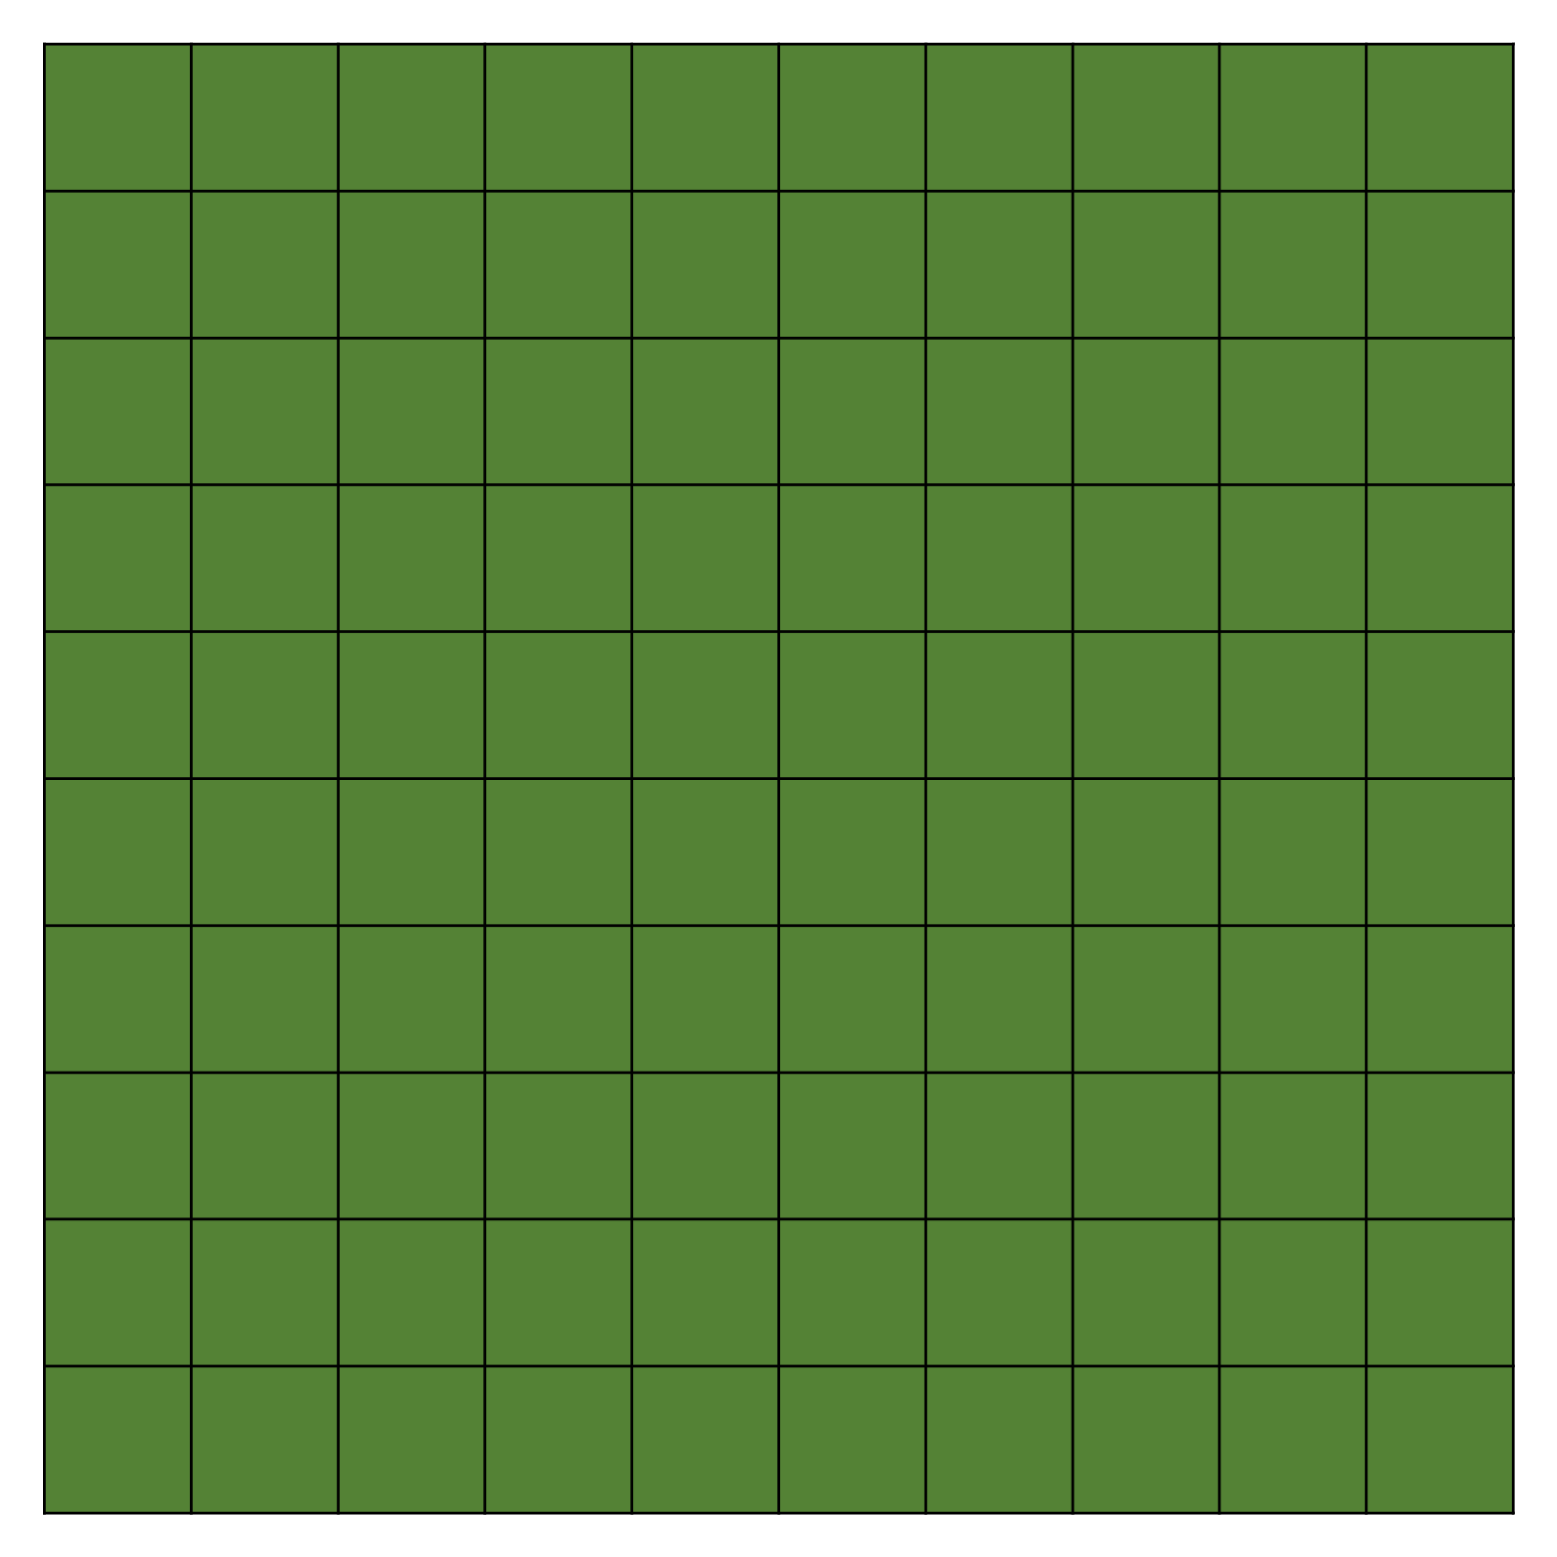
\includegraphics[width=0.4\linewidth]{firebreak/original} 
    \caption{Initial regular graph} 
    \label{fig:original} 
    \vspace{4ex}
  \end{subfigure}%% 
  \begin{subfigure}{0.4\linewidth}
    \centering
    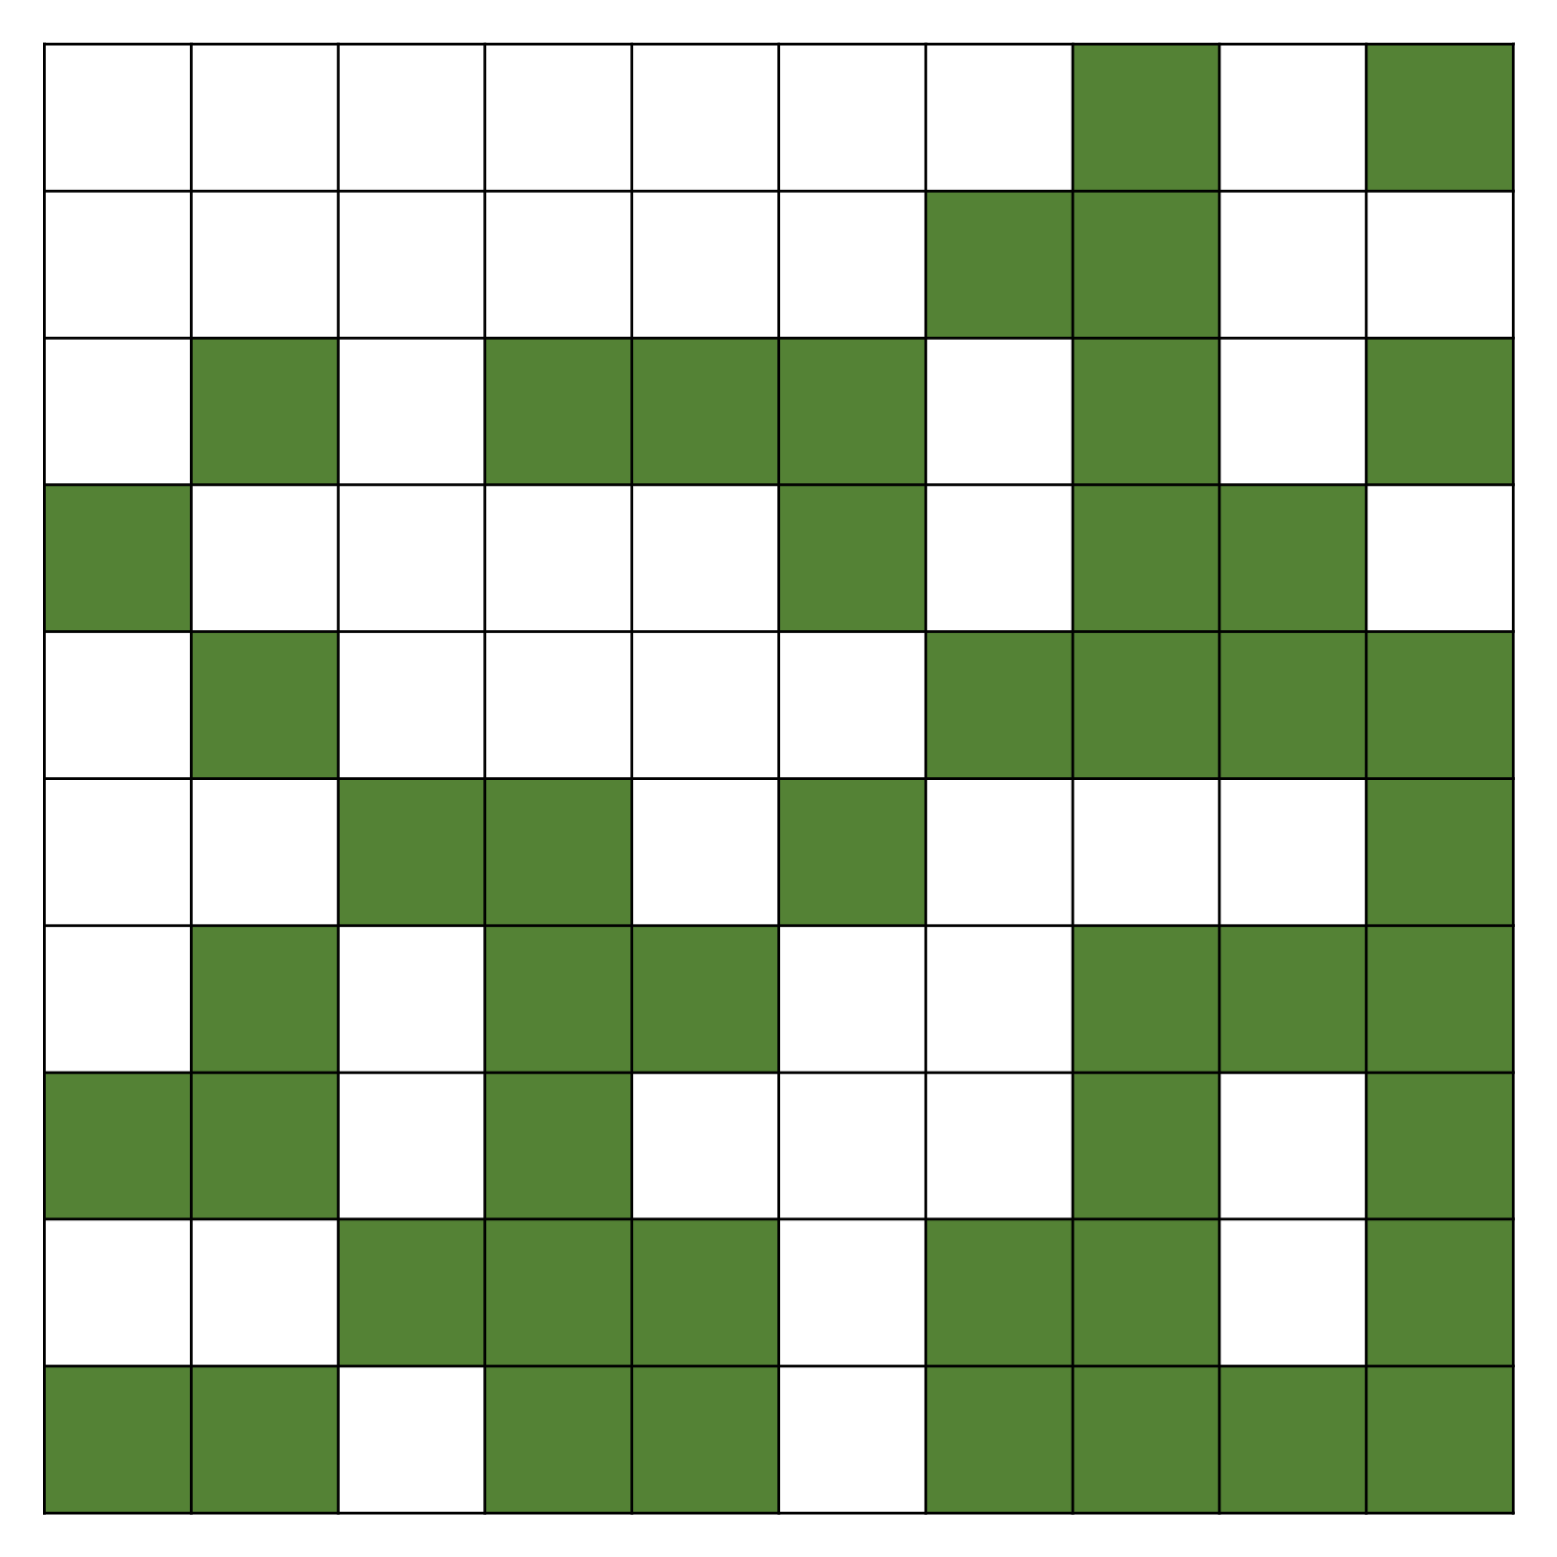
\includegraphics[width=0.4\linewidth]{firebreak/afterperc} 
    \caption{Graph after percolation ($p=1/2$)} 
    \label{fig:afterperc} 
    \vspace{4ex}
  \end{subfigure} 
  \begin{subfigure}{0.4\linewidth}
    \centering
    \includegraphics[width=0.4\linewidth]{firebreak/outbreak} 
    \caption{Initial outbreak ($t=0$)} 
    \label{fig:outbreak} 
  \end{subfigure}%%
  \begin{subfigure}{0.4\linewidth}
    \centering
    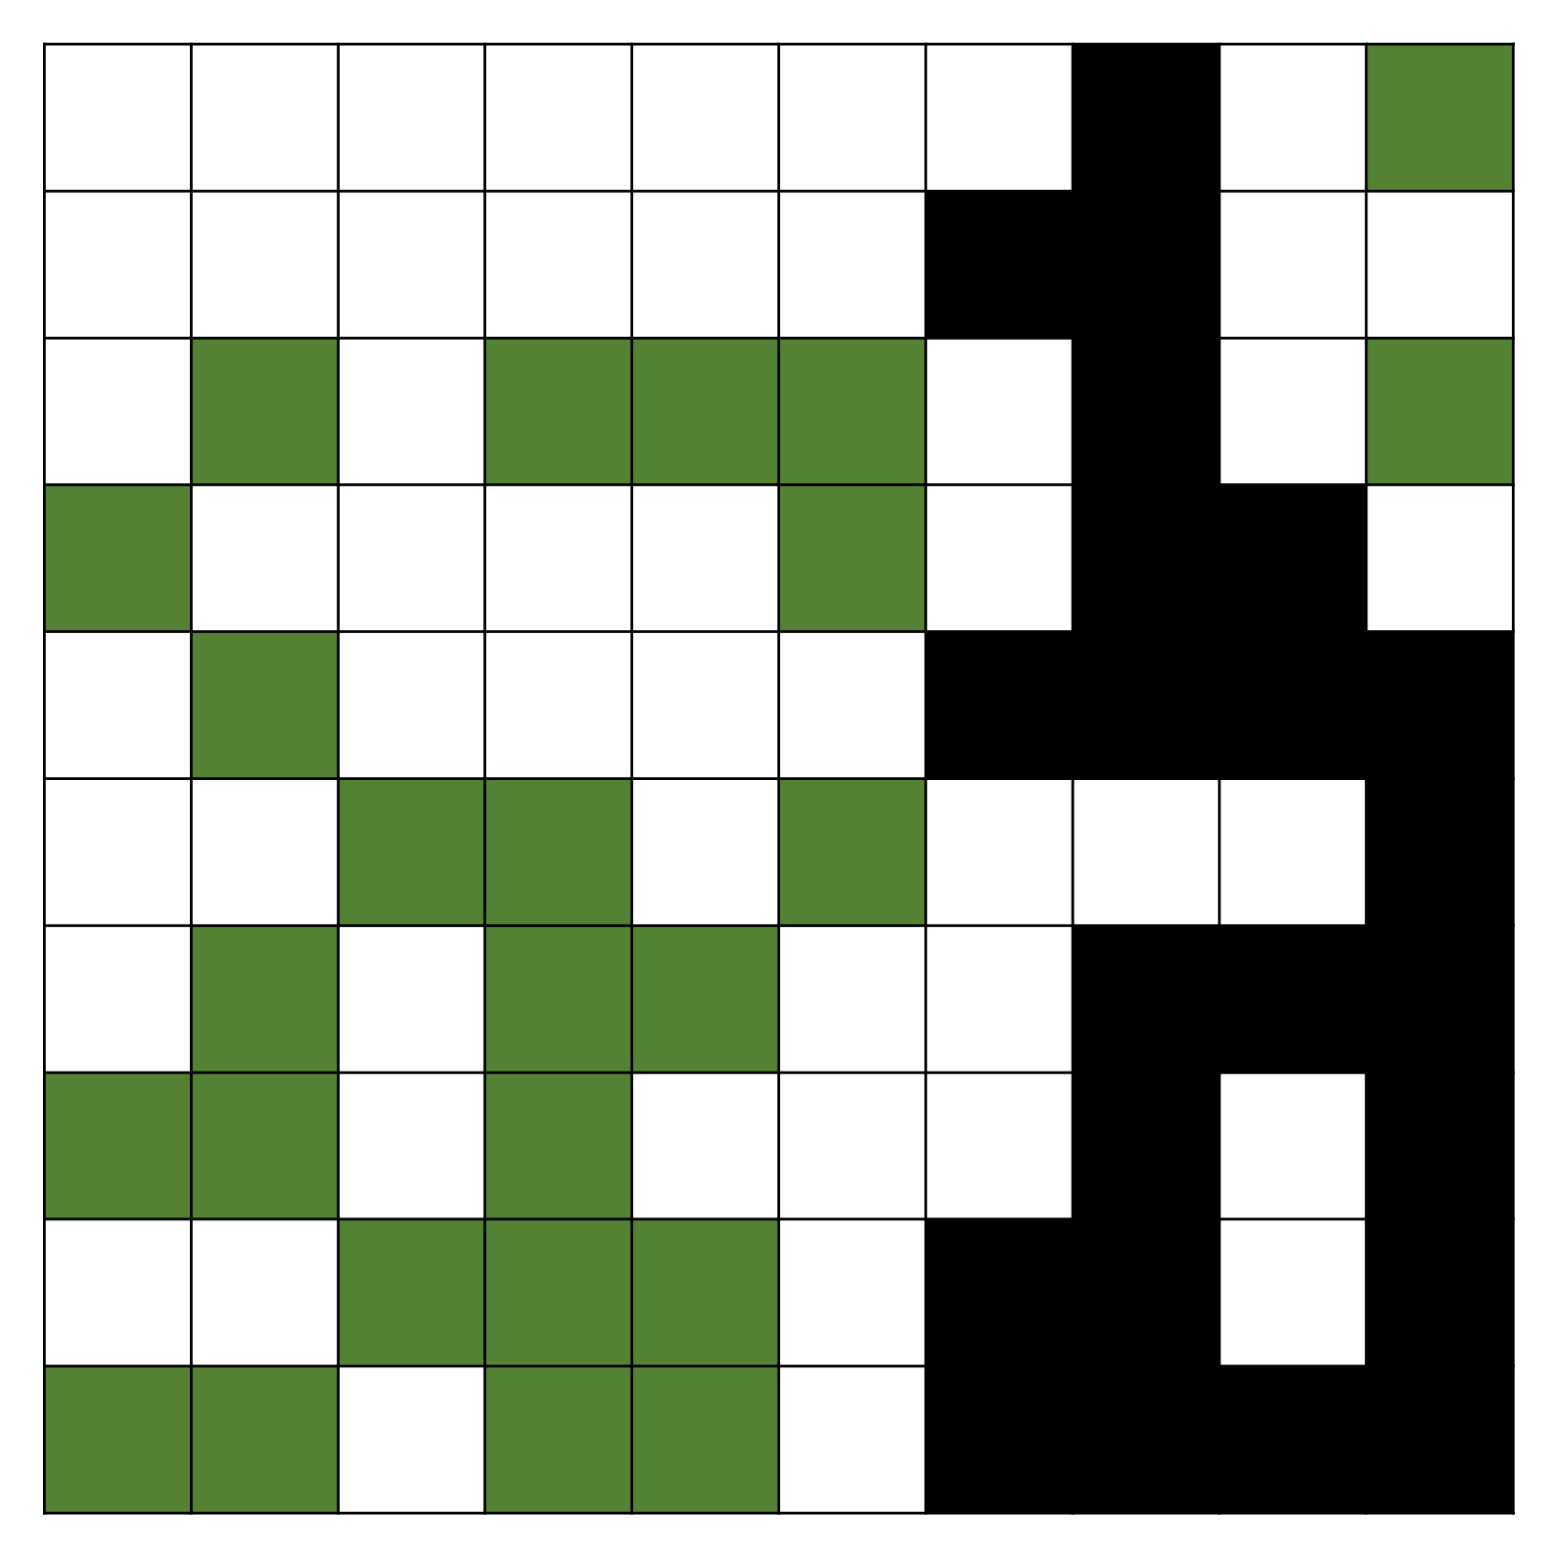
\includegraphics[width=0.4\linewidth]{firebreak/afteroutbreak} 
    \caption{End of outbreak ($t=12$)} 
    \label{fig:end} 
  \end{subfigure} 
  \caption{Outbreak of fire on a percolated graph}
  \label{fig:percolated_graph} 
  \end{centering}
\end{figure}

To illustrate this idea, we will consider a similar (perhaps precursor) to {\scshape Firefighter}, called The Firebreak Problem or simply {\scshape Firebreak}. Rather than have a firefighter reactively combatting the fire on each turn, we begin with an allocated amount of funding with which to mitigate the expected damage of the fire, and spend all of that before the fire begins. Generally, this means we have a number of edges to remove (trees to cut down or place a barrier in between) before the fire begins. Figure \ref{fig:percolated_graph} depicts the use of percolation on a graph to model a forest fire. We can see that the model would have little utility if we began the outbreak on the graph in \ref{fig:original} (all of the graph would be burnt), but percolation has made this a more instructive and realistic model in figure \ref{fig:afterperc}. We can see where the fire has spread in \ref{fig:end}, and we can see where - if we had a finite amount of resources - we must focus our efforts and funding in introducing a firebreak.\\

\begin{figure}[ht] 
\begin{centering}
  \begin{subfigure}{0.4\linewidth}
    \centering
    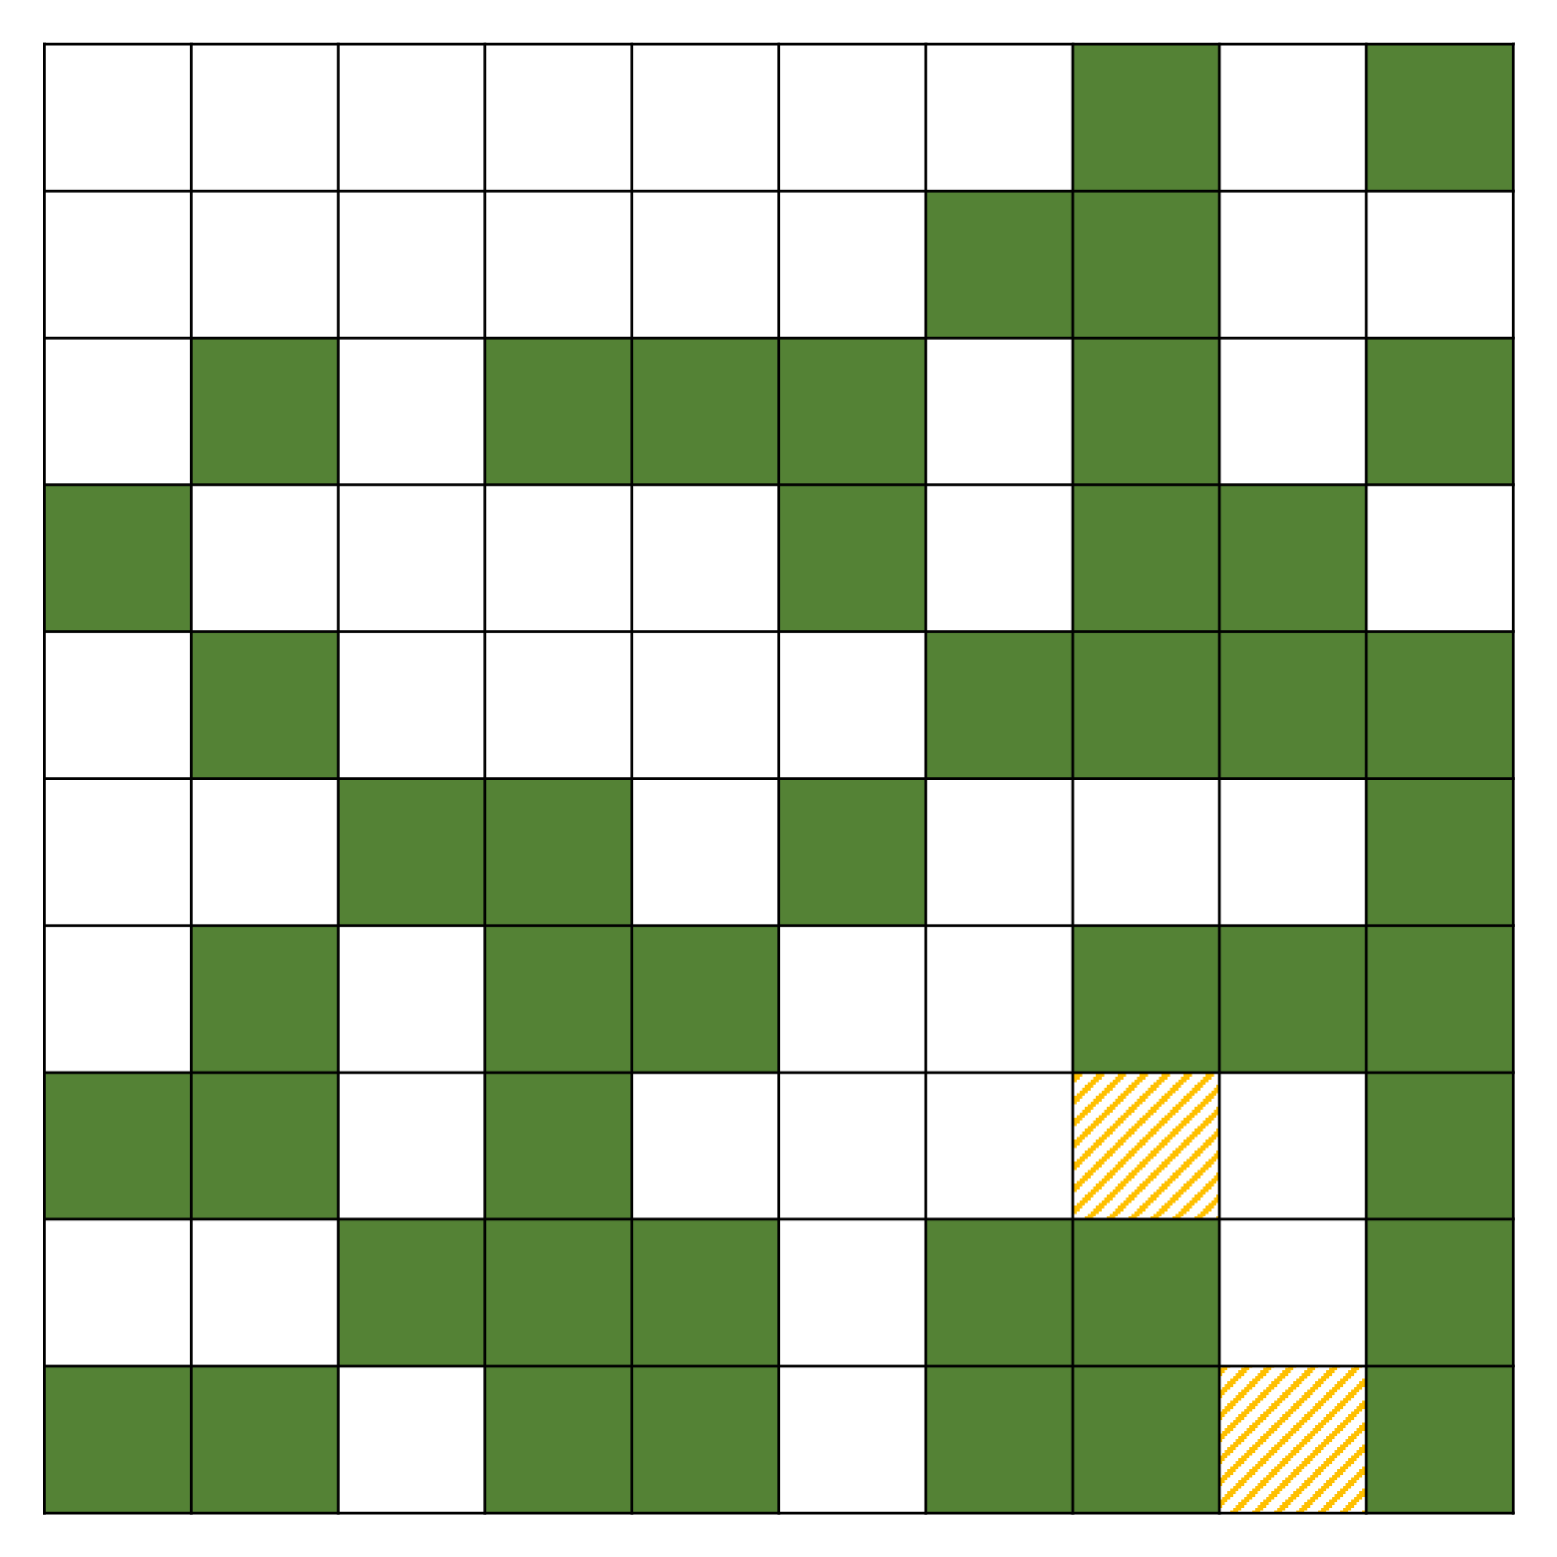
\includegraphics[width=0.4\linewidth]{firebreak/defended/defended} 
    \caption{Position of Firebreak (in yellow)} 
    \label{fig:defended} 
    %\vspace{4ex}
  \end{subfigure}%% 
  \begin{subfigure}{0.4\linewidth}
    \centering
    \includegraphics[width=0.4\linewidth]{firebreak/defended/outbreak} 
    \caption{Fire onset with firebreak ($t=0$)} 
    \label{fig:afterperc_break} 
    %\vspace{4ex}
  \end{subfigure}\\[1ex] 
  \begin{subfigure}{0.4\linewidth}
    \centering
    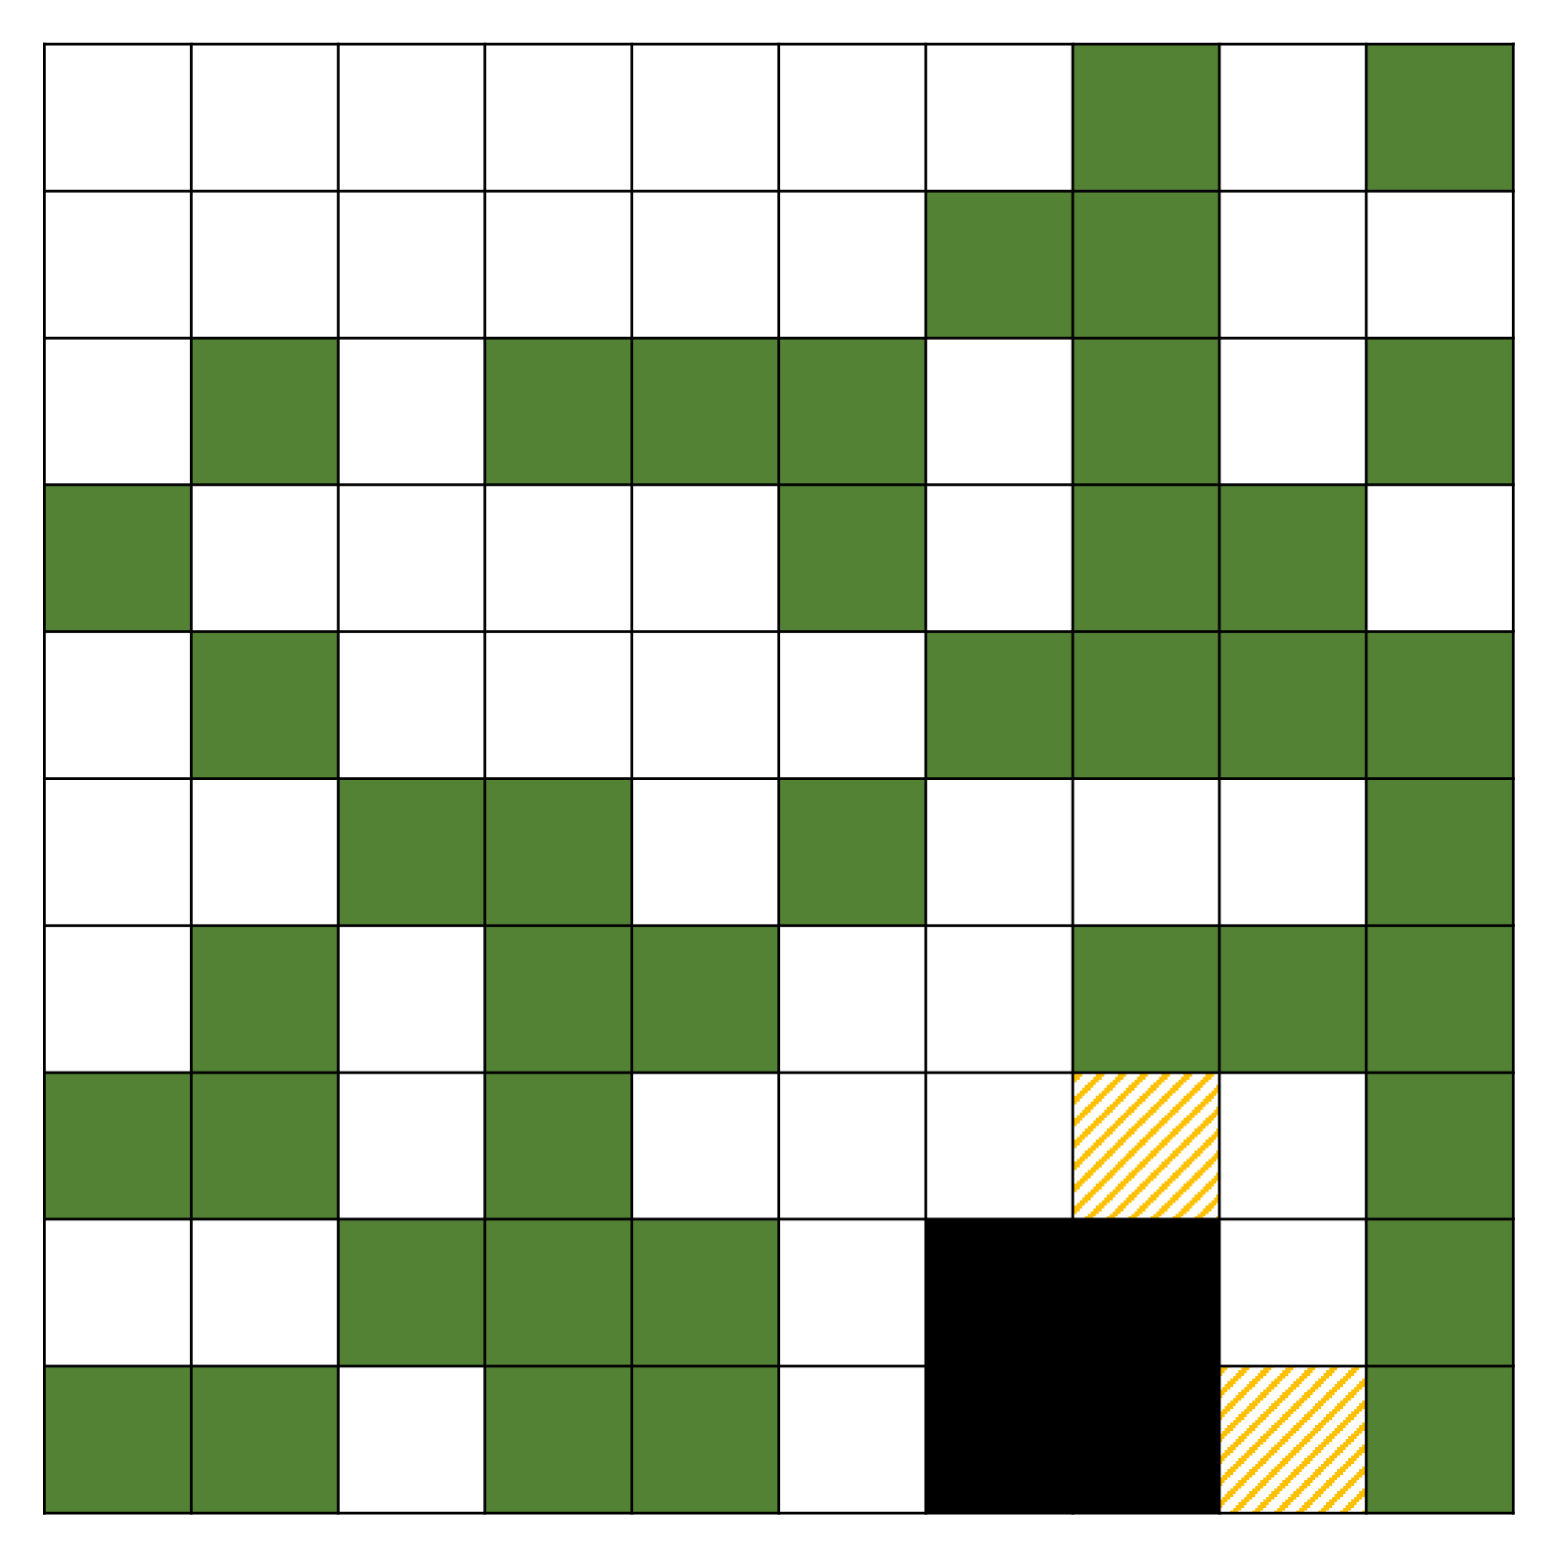
\includegraphics[width=0.4\linewidth]{firebreak/defended/end} 
    \caption{End of outbreak ($t=3$)} 
    \label{fig:end_defended} 
  \end{subfigure} 
  \caption{Outbreak of fire on a defended percolated graph}
  \label{fig:percolated_defended} 
  \end{centering}
\end{figure}

If, for instance, we could only remove two vertices as a firebreak, we ought to make those three the ones shown in yellow in figure \ref{fig:percolated_defended}. This is an example of how percolating a graph for use in {\scshape Firefighter} (and indeed {\scshape Firebreak}) can assist in generating a more realistic and useful model for contagion. There is much interest in the regular graph examples, but our modelling contexts of interest call for a more sporadic graph density and so we, in future research, will try and prove conjectures regarding the minimum number of vertex defences required in {\scshape Firebreak} for percolated graphs of given percolation threshold and dimension (or infinite graphs) and analogous questions in {\scshape Firefighter}.

\subsection{Agency-oriented modelling}

One of the key deficiencies in existing approaches to compartmental models of disease, as described in Section \ref{sec:lit}, is the lack of agency in individuals. To address this, we have designed and implemented (in Java) a compartmental graph model of infectious disease.

In our implemented model, we begin with a graph. This graph has a particular number of vertices and edges and can be generated using code we have written for several random graph types, for instance Erd\H{o}s R\'enyi Barab\'asi–Albert-generated preferential attachment graphs.
% 
%\begin{itemize}
%\item Simple (unweighted, undirected, no loops or multiple edges)
%\item Erd\H{o}s R\'enyi (edge between two vertices exists with given probability)
%\item Complete (every pair of vertices connected by single unique edge)
%\item  Bipartite (vertices can be divided into two, disjoint, independent sets)
%\item Complete bipartite (every pair in each set connected by single unique edge)
%\item Path (graph containing a single path through each vertex)
%\item Binary tree (each vertex has at most three children)
%\item Cycle (graph containing only a single cycle through all vertices)
%\item Eulerian Path (graph containing only a single Eulerian path through all vertices)
%\item Eulerian Cycle (graph containing only a single Eulerian cycle through all vertices)
%\item Wheel (a single vertex connected to every other vertex in a cycle)
%\item Star (a tree with a single internal vertex and a given number of leaves)
%\item Regular (regularly uniform $k$-regular graph)
%\item Tree (uniformly random tree, generated using Pr\"ufer sequence)
%\item A Barab\'asi–Albert-generated preferential attachment graph (can be non-linear)
%\item A Watts-Strogatz model generated small-world graph.
%\end{itemize}

We then assign an agent to each vertex, meaning there is a particular set of agency-related characteristics for each vertex. These characteristics correspond to proximity to infection, their current (compartmental) state and intrinsic inclination towards protection. Agents can be in a number of states, which at the moment are `susceptible' (could contract), `infected' (currently has the infection and is infectious), `recovered' (previously had the infection, may now have some degree of immunity in certain contexts) and `protected' (cannot contract the infection). The final protection-related agent attribute is a novel introduction to the field that we have taken a large amount of time to vary, study and reassess: we term this the `protection rating' of the given vertex. For context, in some infection scenarios this may correspond to how strict the person is with mitigating behaviours to avoid contracting a disease such as hand hygiene, personal protective equipment usage and so on. We can assign this rating purely randomly, based upon proximity to infection or a combination of the two approaches.

\begin{figure}[ht]
  \centering
  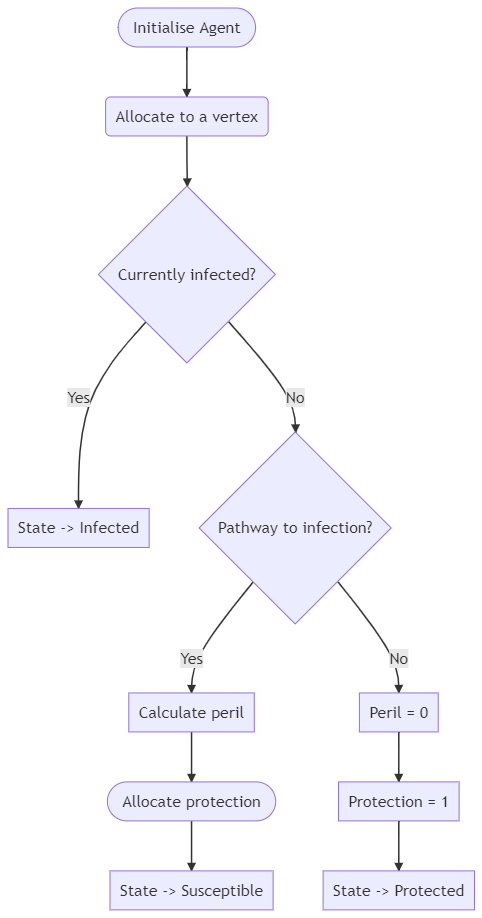
\includegraphics[scale=0.4]{assets/agent-initialisation}
  \caption{Agency initialisation}
  \label{fig:agent}
\end{figure}

\begin{figure}[ht]
  \centering
  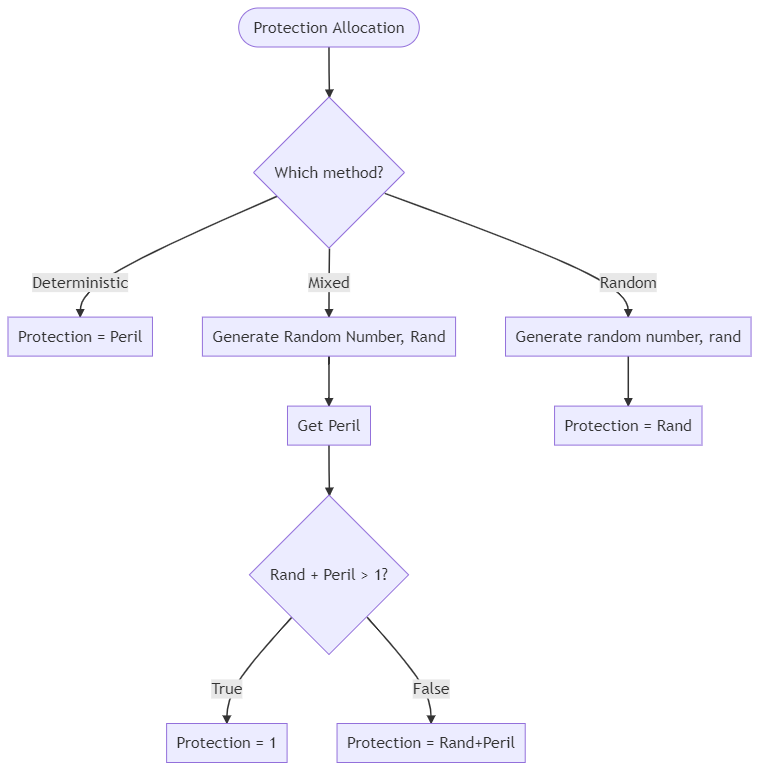
\includegraphics[scale=0.4]{assets/protection}
  \caption{Protection allocation}
  \label{fig:protection}
\end{figure}

Once these agents are initialised, an outbreak (source) vertex is selected from the graph and the agent at that location is moved to the `infected' compartment of the model. Then, a defensive move is made, which is adapted to account for the inherent individual protection ratings. Currently, there are three main defence strategies that are deployed and two further strategies that can be deployed for comparisons.

\begin{figure}[ht]
  \centering
  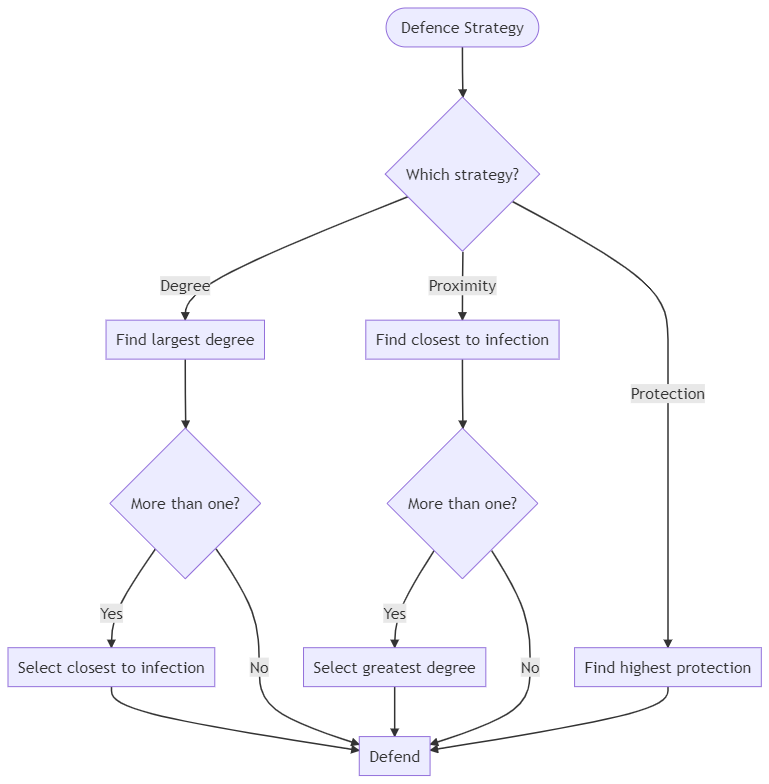
\includegraphics[scale=0.4]{assets/defence}
  \caption{Defence strategies}
  \label{fig:defence}
\end{figure}

\subsection{Equations describing graph-based compartmental models}

\subsubsection{Standard $SIR$ model with fixed population}

The SIR Model is a compartmental epidemiological model with three compartments (generally referred to as `states') related to an epidemic: {\it susceptible, infected} and {\it recovered.} We define $S(t)$ as the number of people who do not currently have but are able to contract the infection at time $t$, $I(t)$ as individuals who currently have the disease and are infectious and finally $R(t)$ as those who have had the disease and subsequently recovered, granting them at least some level of immunity in certain contexts. For a fixed population $N$, we have that $S(t) + I(t) + R(t) = N$ - that is, we assume a fixed population where we do not wish to consider vital dynamics, usually when an epidemic is short-lived. Then, for $\beta$ and $\gamma$ the rates of infection and recovery respectively, the standard SIR model without vital dynamics (birth and death rates) is given as follows:

\begin{align}
\frac{dS}{dt} & = -\beta \frac{SI}{N} \label{dS}\\
\frac{dI}{dt} & = \beta\frac{SI}{N} \gamma I \label{dI}\\
\frac{dR}{dt} & = \gamma I - \mu R \label{dR}
\end{align}

We generally aren't much interested in the expression for $\dot{\langle R \rangle}$, since we require that $ \dot{\langle S \rangle} + \dot{\langle I \rangle} + \dot{\langle R \rangle} = 1$ meaning we can always find the third probability as the compliment of the sum of the other two probabilities. In much of the literature, the convention is for this reason to only give the first two equations.

\subsubsection{Extending the $SIR$ model to graphs}

In order to extend our SIR model to network graphs, we first examine the probability of an agent being in a given class: let $\langle A_i \rangle$ represent the time-independent probability of person $i$ being in state $A$, meaning that the expression of the form $\langle A_i B_i \rangle$ represents the (again, time-independent) probability of individuals $i$ and $j$ being in states $A$ and $B$ respectively \cite{kiss_2014}. We begin with a contact network, where vertices represent individuals and the edges between them represent social contact which may serve as an infection pathway. Then, the adjacency matrix $G$ of this network is constructed by assigning $G_{ij} = 1$ when $i$ and $j$ share an edge and $G_{ij} = 0$ otherwise.\footnote{Because we are infrequently interested in self-transmission, we often set $G_{ii}=0.$} Then, we extend this contact network to a transmission network: let $\beta_i$ represent the per-link infection rate for individual $i$ and $\gamma_i$ represent the recovery rate for $i$. For the transmission matrix $T,$ we assign $T_{ij}=\beta_i$ if there is a route of infection between $i$ and $j$ and $T_{ij}=0$ otherwise. Often, we will consider unweighted and undirected graphs, but in general $T_{ij}$ may not equal $T_{ji}$.\\
We now note that we can replace $\beta_i$ with a term involving such a transmission matrix of a network in order to begin extending the usual SIR model into a network realm. Using the substitution $ \beta_i \frac{SI}{N} = \sum^{N}_{j=1}T_{ij} \langle S_i I_j \rangle,$ the equations become
\begin{align*}
\dot{\langle S_i \rangle} & = -\sum^{N}_{j=1}T_{ij} \langle S_i I_j \rangle\\
\dot{\langle I_i \rangle} & =\sum^{N}_{j=1}T_{ij}\langle S_i I_j \rangle - \gamma_i \langle I \rangle \\
\dot{\langle R_i \rangle} & = \gamma_i \langle I \rangle,
\end{align*}
which are the evolution equations given in \cite{kiss_2014}.

\subsubsection{Adding a new state to the model}

Let $\zeta_i$ be the probability that we defend individual $i$. This can be determined in a number of different ways and we propose that a good candidate for this would be an algorithmic approach.\footnote{That is, determine the best candidates for defence each turn and distribute some given probability across them by the expected benefit in containing the infection gained by defending each vertex.} Similarly, let $\alpha_i$ represent the efficacy of the protection measure for individual $i$, which may decay over time and vary from person to person (for instance, the protection could be more effective in certain age groups than in others). Using these rates of protection and effectiveness, for fixed population size the differential equations become:
\begin{align}
\dot{\langle S_i \rangle} & = \alpha_i \langle P_i \rangle - \sum^{N}_{j=1}T_{ij} \langle S_i I_j \rangle - \zeta_i\langle S_i \rangle\\
\dot{\langle I \rangle} & =\sum^{N}_{j=1}T_{ij}\langle S_i I_j \rangle - \gamma_i \langle I \rangle \\
\dot{\langle R_i \rangle} & = \gamma_i \langle I \rangle \\
\dot{\langle P_i \rangle} & = \zeta_i \langle S_i \rangle - \alpha_i \langle P_i \rangle.
\end{align} 
Accounting for vital dynamics, with a birth and death rate (for simplicity) of $\mu$, these equations are:
\begin{align}
\dot{\langle S_i \rangle} & = \alpha_i \langle P_i \rangle - \sum^{N}_{j=1}T_{ij} \langle S_i I_j \rangle + \mu N - \mu \langle S_i \rangle - \zeta_i\langle S_i \rangle\\
\dot{\langle I \rangle} & =\sum^{N}_{j=1}T_{ij}\langle S_i I_j \rangle - \gamma_i \langle I \rangle - \mu \langle I_i \rangle\\
\dot{\langle R_i \rangle} & = \gamma_i \langle I \rangle + \mu \langle R_i \rangle\\
\dot{\langle P_i \rangle} & = \zeta_i \langle S_i \rangle - \alpha_i \langle P_i \rangle - \mu \langle P_i \rangle.
\end{align}

\subsubsection{Results for total system of equations}

As an example, we consider the `triangle network' - a loop of three nodes. The equations required to precisely express the system $SIR$ dynamics of this network are as follows \cite{kiss_2014}:
\begin{align}
\text{6 singles: } & \dot{\langle S_1 \rangle}, \dot{\langle S_2 \rangle}, \dot{\langle S_3 \rangle}, \dot{\langle I_1 \rangle}, \dot{\langle I_2 \rangle}, \dot{\langle I_3 \rangle}.\label{eq:SIRsingle}\\
\text{6 doubles: } & \dot{\langle S_1 I_2 \rangle},\dot{\langle I_1 S_2 \rangle}, \dot{\langle S_1 I_3 \rangle}, \dot{\langle I_1 S_3 \rangle}, \dot{\langle S_2 I_3\rangle}, \dot{\langle I_2 S_3 \rangle}.\label{eq:SIRdouble}\\
\text{6 triples: } & \dot{\langle S_1 I_2 I_3 \rangle}, \dot{\langle S_1 I_2 S_3 \rangle}, \dot{\langle S_1 S_2 I_3 \rangle}, \dot{\langle I_1 S_2 S_3 \rangle}, \dot{\langle I_1 I_2 S_3 \rangle}, \dot{\langle I_1 S_2 I_3 \rangle}. \label{eq:SIRtriple}
\end{align}
Now, using the equations for the $SIRP$ model, we have the following equation requirements:
\begin{align*}
\text{9 singles: (} \ref{eq:SIRsingle} \text{) and } & \dot{\langle P_1 \rangle}, \dot{\langle P_2 \rangle}, \dot{\langle P_3 \rangle}.\\
\text{18 doubles: (} \ref{eq:SIRdouble} \text{) and }& \dot{\langle S_1 P_2 \rangle},\dot{\langle P_1 S_2 \rangle}, \dot{\langle I_1 P_2 \rangle}, \dot{\langle P_1 I_2 \rangle}, \dot{\langle S_1 P_3\rangle}, \dot{\langle P_1 S_3 \rangle},\\ & \dot{\langle I_1 P_3 \rangle}, \dot{\langle P_1 I_3 \rangle}, \dot{\langle S_2 P_3 \rangle}, \dot{\langle P_2 S_3 \rangle}, \dot{\langle I_2 P_3 \rangle}, \dot{\langle P_2 I_3 \rangle}. \\
\text{24 triples: (} \ref{eq:SIRtriple} \text{) and } & \dot{\langle S_1 S_2 P_3 \rangle}, \dot{\langle S_1 P_2 S_3 \rangle}, \dot{\langle S_1 I_2 P_3\rangle}, \dot{\langle S_1 P_2 I_3 \rangle}, \dot{\langle S_1 P_2 P_3\rangle}, \dot{\langle I_1 S_2 P_3 \rangle},\\
&  \dot{\langle I_1 P_2 S_3 \rangle}, \dot{\langle I_1 I_2 P_3 \rangle}, \dot{\langle I_1 P_2 I_3 \rangle}, \dot{\langle I_1 P_2 P_2 \rangle},  \dot{\langle P_1 S_2 S_3 \rangle}, \dot{\langle P_1 S_2 I_3 \rangle},\\
&  \dot{\langle P_1 I_2 S_3 \rangle}, \dot{\langle P_1 I_2 I_3 \rangle}, \dot{\langle P_1 P_2 I_3 \rangle},  \dot{\langle P_1 P_2 S_3 \rangle}, \dot{\langle P_1 S_2 P_3 \rangle},  \dot{\langle P_1 I_2 P_3\rangle}.
\end{align*}

Note that the reason we dispense with the cases of all three vertices being in the same state is that this would not result in any dynamics - no vertices would ever change state in this case. 

\subsubsection{Implementation}

We have been working on an implementation of the above work in equations generation. Our goal is to produce code that can accept a particular graph, for instance as a CSV file, and determine the number of equations that could be required to fully describe a compartmental model (for instance, $SIR$ or $SIRP$) on that graph. This could be by providing an upper and a lower bound, if the exact graph structure is unknown, or by providing the exact number of equations if the graph is small enough for this to be exactly calculated. Then, with this information, the user can then request the software prints the full list of differential equations that exactly describe the epidemic dynamics using an algorithmic approach to generation. This work is not currently completed, but we aim to have completed this in the coming months when the nuances of closures is fully understood and algorithmically implemented.

\end{document}